\documentclass{article}

\usepackage{float}
\usepackage{graphicx}

\title{Performance Analysis of GPU-Accelerated Optical Flow}
\date{December 8, 2014}
\author{Hari Caushik, Kyle Cesare, Soo-Hyun Yoo}

\begin{document}

\maketitle

\newpage

\tableofcontents

\newpage

\section{Abstract}
GPUs, or graphical processing units, have been shown to have significant
performance speedups in comparison to CPUs for problems or tasks that exhibit
high levels of parallelism. In this project, we investigate differences in
performance metrics between optical flow algorithms run on an Intel Core i5 quad
core CPU and those run on an NVIDIA Jetson TK1 development board. We expected 
the Jetson to run these optical flow algorithms significantly faster due to 
greater parallelism with its GPU. We expect to test the performance on the 
Farneback dense optical flow algorithm. This algorithm will process video frames
captured by a GoPro webcam with a USB interface. The performance metric we will
be measuring is frame processing rate.

\section{Graphical Processing Units (GPUs)}
GPUs have been used to improve the performance of a variety of different 
applications. While CPUs consist of a few powerful cores optimized for 
sequential serial processing, GPUs have a massively parallel architecture 
consisting of thousands of smaller, more efficient cores designed for handling
multiple tasks simultaneously. We expect the optical flow program to run many
orders of magnitude faster on the GPU than on the CPU, as it can process more 
arrays of pixels simultaneously. The Jetson Base Board that we are using 
contains an NVIDIA kepler GPU with 192 CUDA cores.

\section{Optical Flow}
Optical flow is a problem within the field of Computer Vision concerned with 
detecting motion by finding and tracking features or segments across different 
images. Specifically, this involves measuring the motion of specific pixel 
brightness patterns in a sequence of images. Optical flow has many applications
in 3D vision tasks like obstacle avoidance and time-to-collision calculations.
Sparse Optical Flow is the tracking of a few select pixels in a set of images.
Dense Optical Flow is the tracking of all pixels in a set of images, a much more
computationally intensive task.

In this project, we use the Farneback Dense Optical Flow Algorithm, which 
computes a polynomial expansion for a neighborhood of pixels and from that 
polynomial approximation, computes displacement (or motion) fields using linear
algebra. Since the motion fields depend on the size of the neighborhood, 
changing this parameter will produce different motion fields and will probably 
have an effect on the performance of the flow computation.

We will specifically measure the number of frames processed per second using
both platforms. We use OpenCV and its GPU acceleration compiler option to 
implement this program. 
\section{Testing Methodology}
To test the criteria outlined above, we will create two programs to produce
identical outputs, but one will target a CPU and the other a GPU.

To try to identify strengths and weaknesses of each target, we will attempt to
introduce additional variables that may have an impact on performance. These
variables will be:

\begin{description}
  \item[Image resolution] To process a very small image, the overhead required
    to copy memory between the CPU and GPU may be larger than the actual
    processing time. We will use video at QVGA (320x240), VGA (640x480) and FHD
    (1920x1080) to see if this effect is significant.
  \item[Flow magnitude] ?
\end{description}

It is important to note that the processing times for the first few frames will
be discarded to remove any caching oddities and to allow the GPU kernels to
finish load.

\section{Results}

\begin{figure}[H]
  \centering
    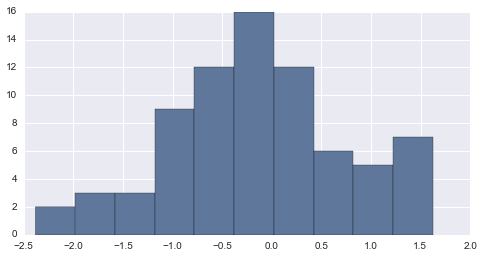
\includegraphics[width=0.8\textwidth]{test_resolution.png}
  \caption{Processing time per frame at various resolutions.}
\end{figure}

\begin{figure}[H]
  \centering
    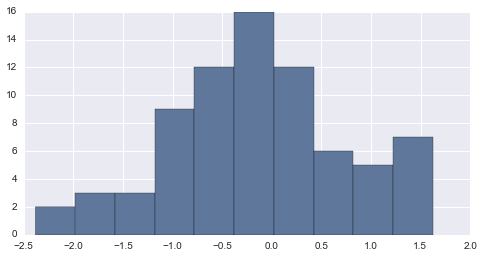
\includegraphics[width=0.8\textwidth]{test_flow.png}
  \caption{Processing time per frame for various magnitudes of motion.}
\end{figure}

\section{Implementation Analysis}
To provide more insight into why the GPU showed better performance results than
the CPU, we will now break down the OpenCV Farneback optical flow implementation
used in the trials. We use the \texttt{objdump} tool to disassemble the OpenCV
shared library into an x86 assembly representation. We then use this assembly
code to gather information on the types and counts of instructions being run.

The heavy use of Streaming SIMD Extensions (SSE) makes it more difficult to
reason about the number of floating point operations being performed.

\section{Conclusion}

\section{Cited Sources}
\begin{thebibliography}{10}
\bibitem{gpuoverview}
http://www.nvidia.com/object/what-is-gpu-computing.html
\bibitem{gpupipeline}
http://www.cs.virginia.edu/~gfx/papers/paper.php?paper_id=59
\bibitem{jetson}
http://www.nvidia.com/object/jetson-tk1-embedded-dev-kit.html
\bibitem{opticalflowgpu}
Real-Time Optical Flow Calculations on FPGA and GPU Architectures: A Comparison
Study
\bibitem{opticalflowtechniques}
wwww.dgp.toronto.edu/~donovan/stabilization/opticalflow.pdf
\bibitem{farneback}
Two-Frame Motion Estimation Based on Polynomial Expansion
\end{thebibliography}
\end{document}
